\documentclass[11pt]{article}

\usepackage[margin=1in]{geometry}
\usepackage{amsmath, amssymb}
\usepackage{graphicx}
\usepackage{subcaption}
\usepackage{booktabs}
\usepackage{placeins}
\usepackage{listings}
\usepackage[colorlinks=true,linkcolor=black,urlcolor=blue,citecolor=black]{hyperref}
\usepackage[capitalise,noabbrev]{cleveref}

\title{\textbf{High Performance Parallel Computing \\ Homework 4: Parallel Tridiagonal Solvers}}
\author{Liam Pohlmann, Alex Shaffer}
\date{\today}

\begin{document}

\maketitle

For this problem, we look at the performance of the parallel tridiagonal solver from class. 
This method decomposes the domain and reorders the system of equation to allow for much of the work to be done in parallel, with the coupling terms from the seperator entries being considered in a second step.


\subsection*{Verification}
It doesn't matter how fast the solver works if it doesn't actually solve the problem.
In~\cref{tab:verify}, we copute the residual, relative residual, and error for a known solution $x_{\text{true}}$.
All of these are on the order of machine precision, which is what we expect for a fucntioning solver with a well-conditioned matrix.


\begin{table}[htbp]
  \centering
  \caption{Verification of the domain-decomposition solver against a known solution $x_{\text{true}}$, with $f = A x_{\text{true}}$.
    Each row reports the worst value over 3 trials, each with a new random matrix and right-hand side.}
  \label{tab:verify}
  \begin{tabular}{rrccc}
    \toprule
    $P$ & $N$ & $\|f - Ax\|_\infty$ & $\|f - Ax\|_2 / \|f\|_2$ & $\|x - x_{\text{true}}\|_\infty$ \\
    \midrule
     1 & 128     & $1.665\times10^{-16}$ & $9.890\times10^{-17}$ & $2.220\times10^{-16}$ \\
     2 & 128     & $2.220\times10^{-16}$ & $1.008\times10^{-16}$ & $2.220\times10^{-16}$ \\
     4 & 128     & $1.943\times10^{-16}$ & $1.232\times10^{-16}$ & $2.776\times10^{-16}$ \\
    16 & 128     & $2.776\times10^{-16}$ & $1.181\times10^{-16}$ & $2.776\times10^{-16}$ \\
    64 & 128     & $1.943\times10^{-16}$ & $1.148\times10^{-16}$ & $2.220\times10^{-16}$ \\
    \midrule
     1 & 1000    & $2.776\times10^{-16}$ & $9.738\times10^{-17}$ & $5.551\times10^{-16}$ \\
     2 & 1000    & $2.776\times10^{-16}$ & $9.756\times10^{-17}$ & $5.551\times10^{-16}$ \\
     4 & 1000    & $2.776\times10^{-16}$ & $9.854\times10^{-17}$ & $5.551\times10^{-16}$ \\
    16 & 1000    & $2.776\times10^{-16}$ & $1.051\times10^{-16}$ & $4.441\times10^{-16}$ \\
    64 & 1000    & $3.053\times10^{-16}$ & $1.165\times10^{-16}$ & $4.441\times10^{-16}$ \\
    \midrule
     1 & 65536   & $3.886\times10^{-16}$ & $9.218\times10^{-17}$ & $5.551\times10^{-16}$ \\
     2 & 65536   & $3.886\times10^{-16}$ & $9.221\times10^{-17}$ & $5.551\times10^{-16}$ \\
     4 & 65536   & $3.886\times10^{-16}$ & $9.218\times10^{-17}$ & $5.551\times10^{-16}$ \\
    16 & 65536   & $3.886\times10^{-16}$ & $9.228\times10^{-17}$ & $5.551\times10^{-16}$ \\
    64 & 65536   & $4.441\times10^{-16}$ & $9.283\times10^{-17}$ & $5.551\times10^{-16}$ \\
    \midrule
     1 & 1048576 & $4.441\times10^{-16}$ & $9.180\times10^{-17}$ & $1.055\times10^{-15}$ \\
     2 & 1048576 & $4.441\times10^{-16}$ & $9.180\times10^{-17}$ & $1.055\times10^{-15}$ \\
     4 & 1048576 & $4.441\times10^{-16}$ & $9.180\times10^{-17}$ & $1.055\times10^{-15}$ \\
    16 & 1048576 & $4.441\times10^{-16}$ & $9.181\times10^{-17}$ & $1.055\times10^{-15}$ \\
    64 & 1048576 & $4.441\times10^{-16}$ & $9.184\times10^{-17}$ & $1.055\times10^{-15}$ \\
    \bottomrule
  \end{tabular}
\end{table}

\subsection*{Performance Analysis}
To understand the parallel performance of our solver we do both strong and weak scaling studies.
All of these runs use L3 cache mapping to try and decouple memeory contention from the rest of the parallel performance.
Without L3 cache mapping, we generally see the intra node efficiency degrade more substantially earlier on.



\subsubsection*{Strong Scaling}
For our strong scaling problem we choose a problem large enough to see the overarching trends.
\cref{fig:strong} shows the time to solution in~\cref{fig:strong_time}, the speedup in~\cref{fig:strong_speedup}, and the parallel efficiency in~\cref{fig:strong_efficiency}.
We see largely the expected trends, with the time to solution decreasing nearly linearly with the number of processors. 
There are a couple interessting features of these graphs. First, we see an initial superlinear speedup.
This is due to cache effects. This makes sense because with a tridiagonal matrix, the enties used for the operations fit well into cache. 
This is particularly notable due to the manner in which processors on a node are filled. The L3 cache mapping emphasizes the cache effects.
This is also visible in the speedup and parallel efficiency plots.
Second, we see the speedup plateau between 32 and 128 ranks and then continue roughly linearly.
This is due to the 128 rank nodes that were used. Memory contention comes into play as we fill the first node, but then speedups are realized when we move onto the second node.
We cross the 80\% parallel efficiency threshold between 32 and 64 ranks.


\begin{figure}[htbp]
  \centering
  \begin{subfigure}{0.32\textwidth}
    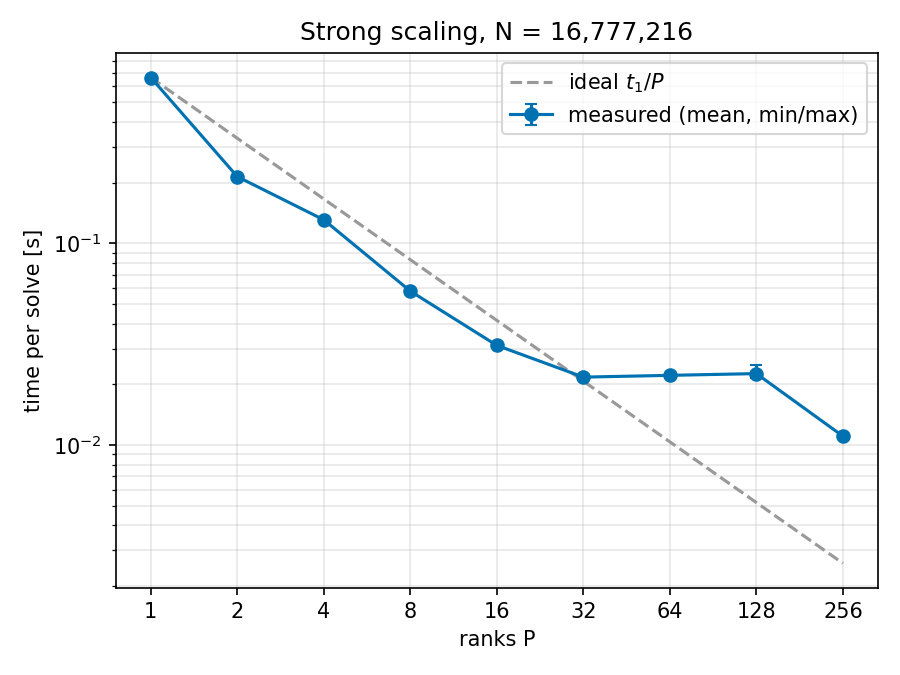
\includegraphics[width=\linewidth]{figures/strong_time.png}
    \caption{Time}
    \label{fig:strong_time}
  \end{subfigure}
  \hfill
  \begin{subfigure}{0.32\textwidth}
    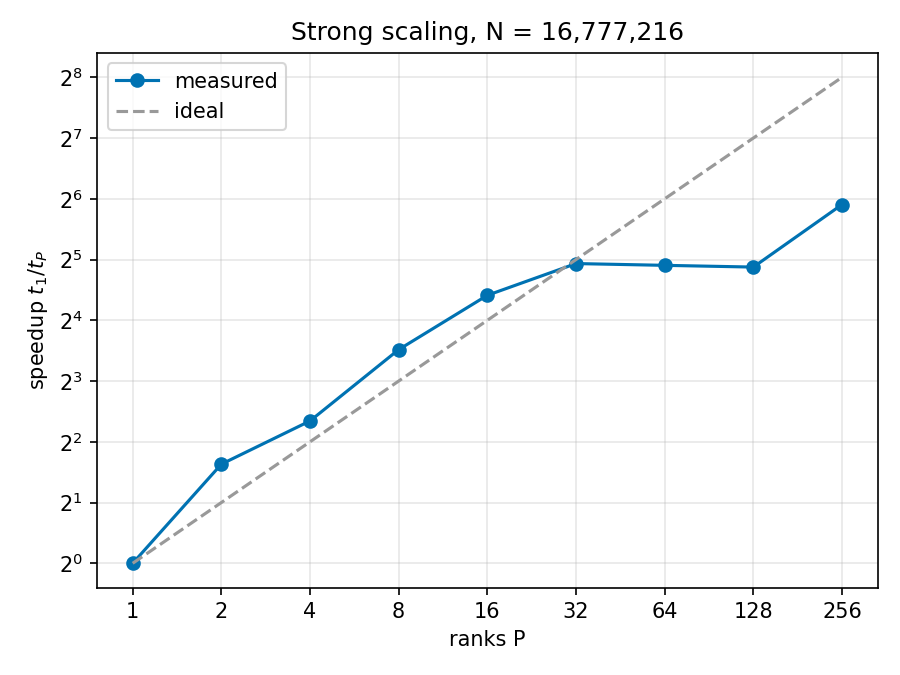
\includegraphics[width=\linewidth]{figures/strong_speedup.png}
    \caption{Speedup}
    \label{fig:strong_speedup}
  \end{subfigure}
  \hfill
  \begin{subfigure}{0.32\textwidth}
    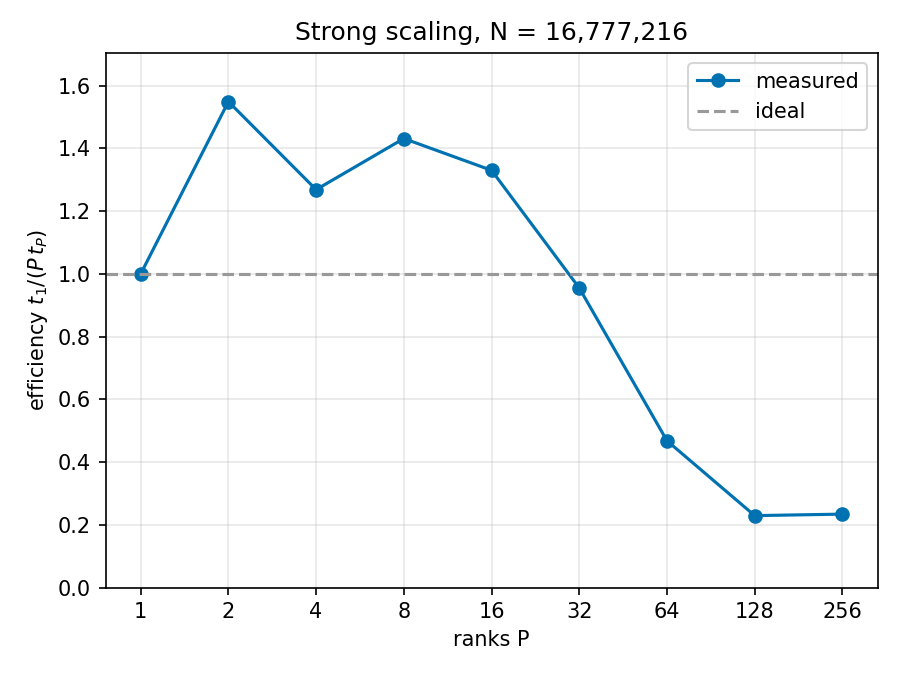
\includegraphics[width=\linewidth]{figures/strong_efficiency.png}
    \caption{Efficiency}
    \label{fig:strong_efficiency}
  \end{subfigure}
  \caption{Strong scaling.}
  \label{fig:strong}
\end{figure}

\subsection*{Weak Scaling}
Weak scaling tells a similar story.~\cref{fig:weak} shows near perfect weak scaling up to 32 ranks, where the memory contention then starts to take effect.
One difference is that we measure the number of GFLOPS in~\cref{fig:weak_gflops}. The ammout of work we can do follows the same trend as the solve time and speedup.
This suggests, I believe, that the memory contention is one of the biggest players in this algorithm, as compared the the communication that occurs in the Schur complement update.
We see 80\% parallel efficiency in the occur in the same region as the strong scaling.

\begin{figure}[htbp]
  \centering
  \begin{subfigure}{0.32\textwidth}
    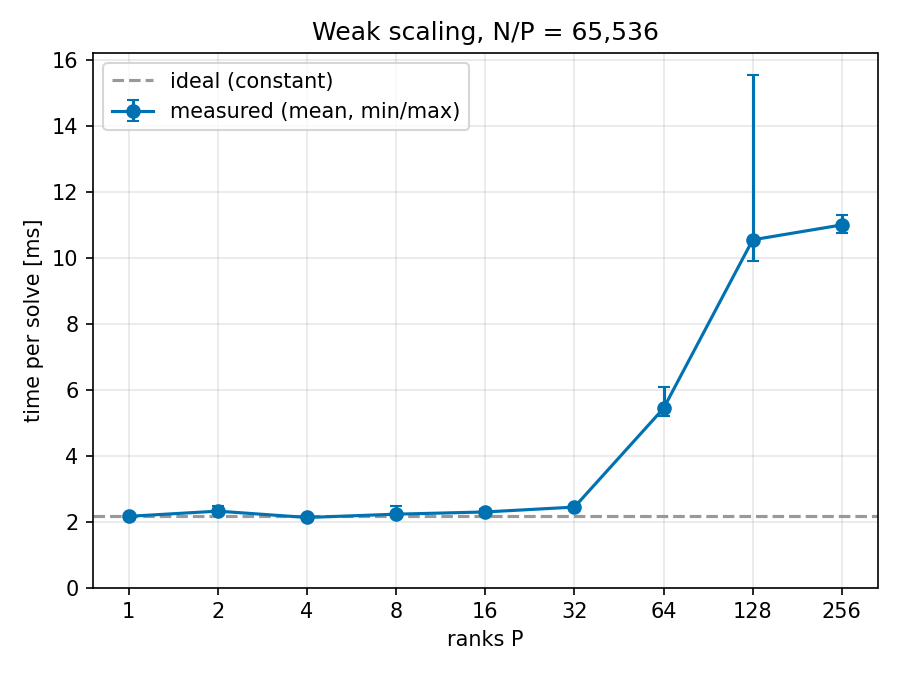
\includegraphics[width=\linewidth]{figures/weak_time.png}
    \caption{Time}
    \label{fig:weak_time}
  \end{subfigure}
  \hfill
  \begin{subfigure}{0.32\textwidth}
    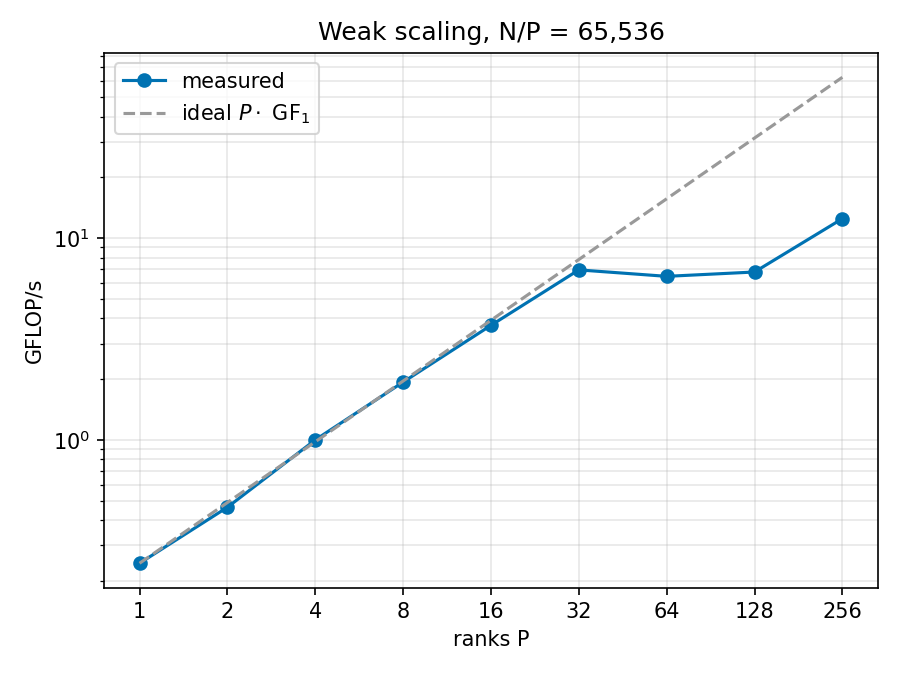
\includegraphics[width=\linewidth]{figures/weak_gflops.png}
    \caption{GFLOP/s}
    \label{fig:weak_gflops}
  \end{subfigure}
  \hfill
  \begin{subfigure}{0.32\textwidth}
    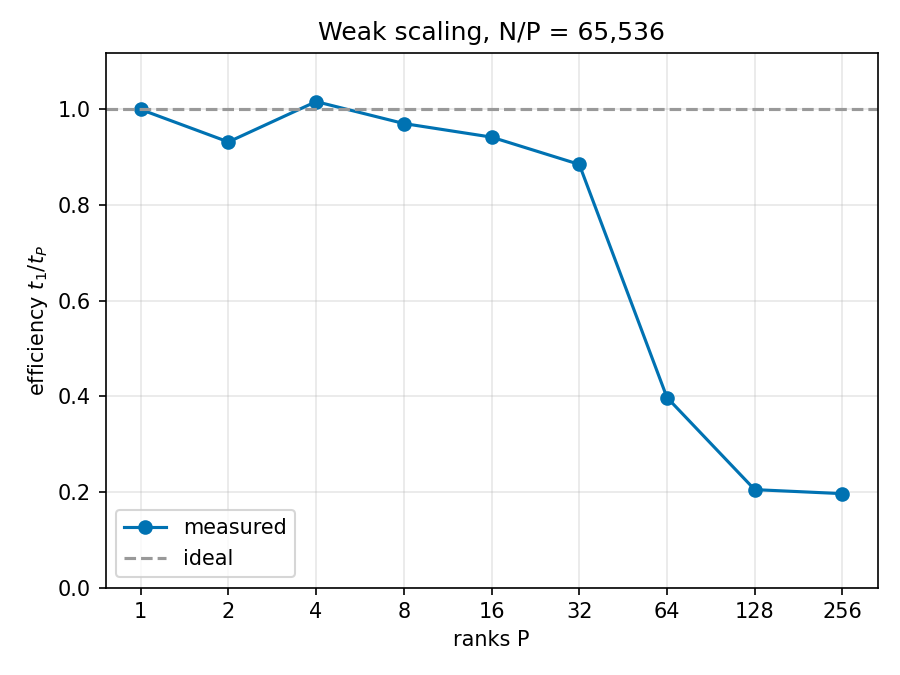
\includegraphics[width=\linewidth]{figures/weak_efficiency.png}
    \caption{Efficiency}
    \label{fig:weak_efficiency}
  \end{subfigure}
  \caption{Weak scaling.}
  \label{fig:weak}
\end{figure}

\clearpage
\appendix
\section{Schur Complement Solver}
This is the c code for our tridiagonal solver. We originally wrote this in c++, but then asked Claude to convert it to C. Timings between the two languages were essentially the same, but all timings in this report were from the c version.
\lstinputlisting[language=C, basicstyle=\ttfamily\footnotesize, numbers=left, numberstyle=\tiny, columns=fullflexible, keepspaces=true, showstringspaces=false, breaklines=true]{../c/src/tridiag.c}

\end{document}
